\documentclass[lettersize,journal]{IEEEtran}
\usepackage{amsmath,amsfonts}
\usepackage{algorithmic}
\usepackage{algorithm}
\usepackage{array}
\usepackage[caption=false,font=normalsize,labelfont=sf,textfont=sf]{subfig}
\usepackage{textcomp}
\usepackage{stfloats}
\usepackage{url}
\usepackage{multicol}
\usepackage{multirow}
\usepackage{verbatim}
\usepackage[utf8]{inputenc}
\usepackage{graphicx}
\usepackage{cite}
\hyphenation{op-tical net-works semi-conduc-tor IEEE-Xplore}
% updated with editorial comments 8/9/2021

% Aditional

\usepackage{hyperref}
	
	\hypersetup{
    colorlinks=true,
    linkcolor=black,
    filecolor=black,      
    urlcolor=black,
    citecolor=black
	}

	\urlstyle{same}

\usepackage{caption}
\captionsetup{justification=centering}


\begin{document}

\title{Radar System for Cardiopulmonary Sensing}

\author{Julio Sebastian Diaz León (judiazl@unal.edu.co)\\Omar Ferney Alvarez Herrera (oalvarezh@unal.edu.co) \\ Esteban Ladino Fajardo (eladinof@unal.edu.co) \\Sergio Andrés Lozano Avila (sealozanoa@unal.edu.co)\\

\IEEEauthorblockA{\IEEEmembership{Radar Systems}}

Universidad Nacional de Colombia

}
        % <-this % stops a space


% The paper headers
\markboth{Radar Systems - Proyect Proposal - October 2023}%
{Shell \MakeLowercase{\textit{et al.}}: A Sample Article Using IEEEtran.cls for IEEE Journals}

%\IEEEpubid{0000--0000/00\$00.00~\copyright~2021 IEEE}
% Remember, if you use this you must call \IEEEpubidadjcol in the second
% column for its text to clear the IEEEpubid mark.

\maketitle

\begin{abstract}
In biomedical industry, there have been some explorations as radar technologies are concerned. One of those applications involves monitoring vital signs. This document shows problem statement and proposed solution for a radar system intended to measure heartbeat and respiration rate given a list of specifications which have to be met in order to ensure its best performance. related work on this topic is included as well as an action plan to be executed. 
\end{abstract}

\begin{IEEEkeywords}
Cardiology, Electronic healthcare, Health and safety, Pulmonology, Radar antennas, Radar detection, Radar measurements, Radar signal processing, Wearable Health Monitoring Systems.
\end{IEEEkeywords}


\section{Interest of the system developed, applications and previous works}


Radar systems are a widely recognized technology in constant development across various fields, including healthcare. Specifically, for cardiopulmonary sensing, it represents a technological innovation with the potential to revolutionize medical monitoring and patient care in various healthcare settings. Its development has generated significant interest both within the medical community and the technology industry, owing to its potential applications and its capacity to enhance healthcare.\\


The primary focus of the developed system lies in its non-invasive capability to detect and monitor vital signs \cite{luAccurateHeartBeat2023a}, such as heart rate and respiration, using radar waves. This eliminates the need for sensors or devices requiring direct skin contact, enabling continuous and precise patient monitoring. This is particularly beneficial in critical environments such as intensive care units, for example, in the case of burn patients \cite{luAccurateHeartBeat2023a}.\\

The applications of this system are diverse, spanning from healthcare in hospitals to remote patient monitoring in homes, leveraging high-speed internet connections via fiber optics and even 5G, integrating IoT monitoring systems for data transmission to healthcare centers and specialists. Moreover, it can be employed for early detection of abnormal cardiac and respiratory events, which is crucial for preventive care and the development of public health policies focused on prevention.\\

There is a substantial body of articles, conferences, and reviews that demonstrate a keen interest in the use of this technology and show significant progress in the field. Prototypes have been implemented with humans, yielding tangible and consistent results when compared to well-established methods, such as electrocardiography, sensors, and even smartwatches equipped with optical sensors.\\

Returning to an initial article that refers to algorithms for detecting vital signs, we can mention "Ultra-wide band impulse radar for life detection using wavelet packet decomposition," \cite{LIANG201831} published in the Journal Physical Communication by ScienceDirect. This article presents an improved algorithm for life detection using ultra-wide band impulse radar (UWB) \cite{kakouche}through walls. Although in our project development, we aim for scenarios without obstacles in transmission or reception, this condition is worth considering. It contributes to the state of the art in the field, as it can detect cardiac and respiratory movements. The algorithm analyzes variations in collected pulses, which are influenced by factors such as time of arrival (TOA) between the UWB radar and the human subject, calculated through wavelet packet decomposition. Frequencies of human cardiac and respiratory movements are collected through a variable time window (VTW).\\

A second article to consider is presented at the IEEE Radio and Wireless Symposium (RWS) 2023, titled "Accurate Heart Beat Detection with Doppler Radar using Bidirectional GRU Network."\cite{luAccurateHeartBeat2023a} This article offers insights into the use of neural networks for obtaining vital signs through a Doppler radar, potentially making it a valuable choice for our project. It also considers continuous wave (CW) radar, where the signal processing involves a four-stage method: baseband signal collection, Butterworth filtering, noise elimination, and the application of a neural network model.\\


A third document worth mentioning is "Super-Regenerative Oscillator Based High-Sensitivity Radar Architecture for Motion Sensing and Vital Sign Detection,"\cite{yuanSuperregenerativeOscillatorbasedHighsensitivity2021} published in IEEE Transactions on Microwave Theory and Techniques. Its major contribution to the state of the art lies in establishing a functional architecture for radar system implementation, incorporating a component called the super-regenerative oscillator (SRO) and a 2.32 GHz patch antenna. As a complementary aspect to the project's development, it addresses the absence of RF signal generators, offering an alternative that doesn't rely on software-defined radios like USRP, potentially reducing costs.\\

With a radar system is possible measurements several patient vital signs and it is necessary to identify other sources as human movements \cite{f.kraiemDopplerRadarArchitecture2019}. Other contactless methods as thermal imagining, infrared thermography equipment, and video imaging have problems in implementation to the cost or physics requirements \cite{f.kraiemDopplerRadarArchitecture2019}. The radars can also be used to search for survivors in disasters and control security areas \cite{f.kraiemDopplerRadarArchitecture2019}.        



\section{Problem statement and specifications}

The main objective of this project is to develop a system capable of measuring heartbeat and respiration rates. In order to assess its quality, there are some specifications that radar system must fulfil as follows:

\begin{enumerate}
    \item System's spectrum usage must comply applicable law.
    \item Measurement distance from subject must be from 0 to 2 meters.
    \item Real-time operation, heart rate and respiration rate display at most ten seconds after the positioning of the subject in front of the radar.
    \item System must include indication of the presence or absence of a subject.
    \item Maximum measurement error: 20\% for both heart and respiratory rates.
    \item False alarm rate of subject presence less than 20\%.
    \item Detection rate of subject presence 70\%.
\end{enumerate}



\section{Project Planning}

In this section, planning method is explained including list of activities, a schedule for project development and a state of advance of ongoing tasks. 

\subsection{List Of Activities}

We have designed list of activities as follows:

% Please add the following required packages to your document preamble:
% \usepackage{graphicx}
\begin{table}[H]
\centering
\caption{Project List of Activities}
\label{tab:activities}
\resizebox{\columnwidth}{!}{%
\begin{tabular}{|r|l|l|l|}
\hline
 ID        & Task Name                                & Start Date      & Due Date        \\ \hline
1              & Radar System for Cardiopulmonary Sensing & 18-Sep          & 1-Dec           \\ \hline
\textbf{1.1}   & \textbf{Project Kick-Off}                & \textbf{19-Sep} & \textbf{19-Sep} \\ \hline
1.2            & Bibliographical Review                   & 19-Sep          & 12-Oct          \\ \hline
1.3            & Architecture Design                      & 24-Sep          & 17-Oct          \\ \hline
\textbf{1.4}   & \textbf{Project Proposal}                & \textbf{17-Oct} & \textbf{17-Oct} \\ \hline
1.5            & System Prototyping                       & 28-Sep          & 23-Nov          \\ \hline
1.5.1          & Antenna Design (v1.0)                    & 28-Sep          & 11-Oct          \\ \hline
1.5.2          & Antenna 1.0                              & 11-Oct          & 23-Oct          \\ \hline
\textbf{1.5.3} & \textbf{System Prototype V1.0}           & \textbf{3-Nov}  & \textbf{3-Nov}  \\ \hline
1.5.4          & Processing Module Design                 & 18-Oct          & 29-Oct          \\ \hline
1.5.5          & Phantom Construction                     & 18-Oct          & 25-Oct          \\ \hline
\textbf{1.5.6} & \textbf{Phantom V1.0}                    & \textbf{27-Oct} & \textbf{27-Oct} \\ \hline
1.5.7          & Prototype Enhancements                   & 6-Nov           & 24-Nov          \\ \hline
\textbf{1.5.8} & \textbf{Final Prototype}                 & \textbf{30-Nov} & \textbf{30-Nov} \\ \hline
1.6            & System Testing                           & 6-Nov           & 24-Nov          \\ \hline
1.7            & Results Analysis                         & 15-Nov          & 30-Nov          \\ \hline
\textbf{1.8}   & \textbf{Final Report}                    & \textbf{1-Dec}  & \textbf{1-Dec}  \\ \hline
\textbf{1.9}   & \textbf{Project Closure}                 & \textbf{1-Dec}  & \textbf{1-Dec}  \\ \hline
\end{tabular}%
}
\end{table}

Note that there are two main topics: Information Gathering and Prototyping. This list of activities can be displayed in a better way through Gantt Diagram as shown in fig. \ref{fig:Gantt}

\begin{figure}[h!]
    \centering
    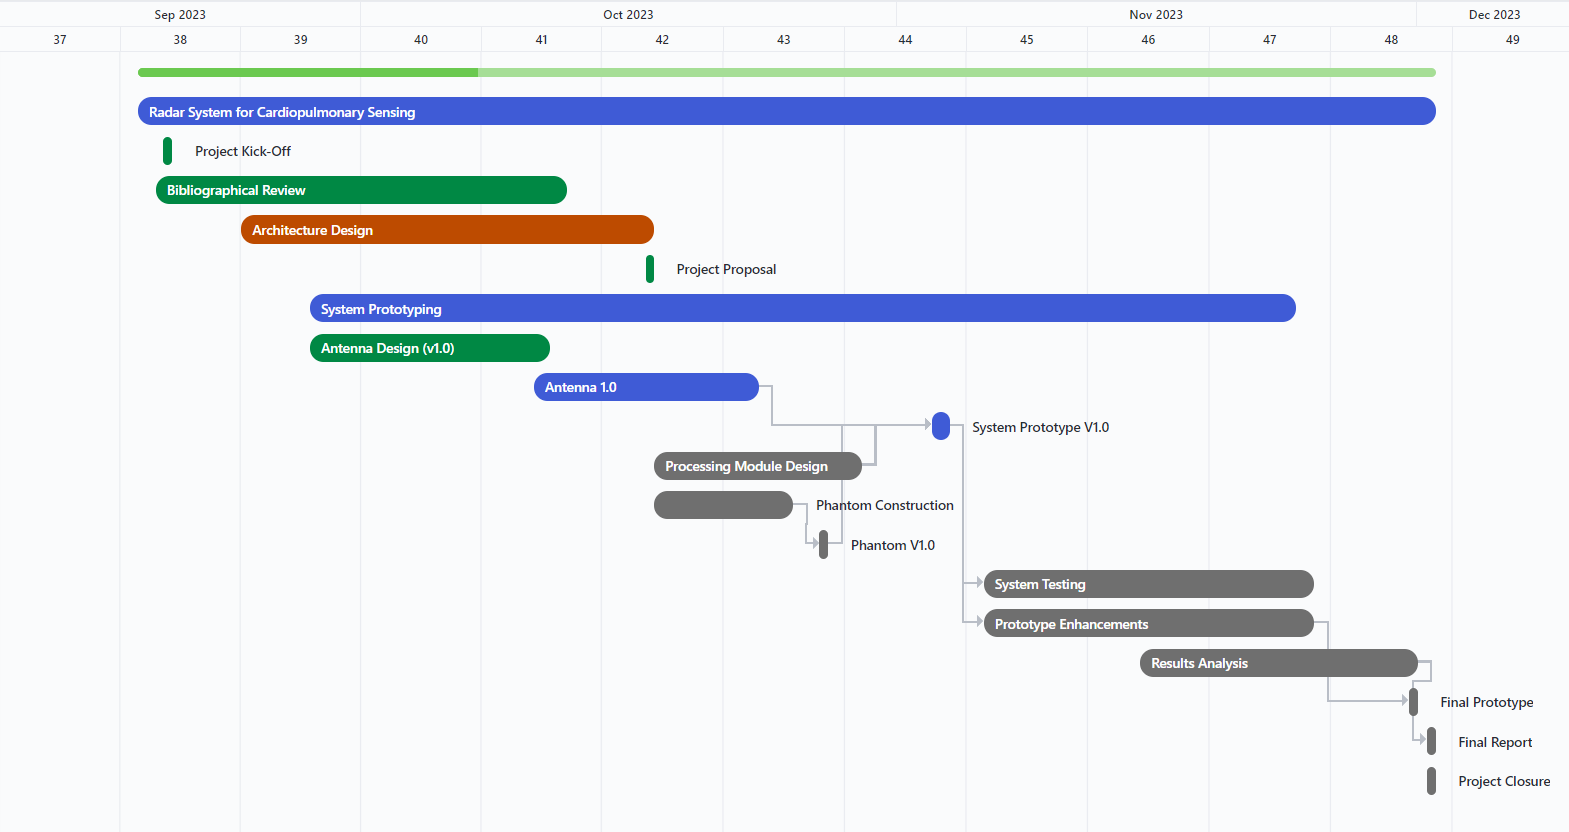
\includegraphics[scale=0.17]{figs/Gantt.png}
    \caption{Project Gantt Chart}
    \label{fig:Gantt}
\end{figure}
 
Gantt Chart shows status of advance of each one of the related activities using the following conventions: Green represents completed activities; Blue, in progress; orange, reviewing; and black, to do. Given that, we can see that main advances reported at the moment this document is presented are essentially the bibliographic review and a first antenna design as it is explained in section \ref{sec:prel_res}. 
Currently, architecture design is under assessment as there are three proposed alternatives: a Doppler-Effect Continuous Wave radar, a Frequency-modulated Continuous Wave radar and an Ultra Wideband Pulse Radar. In that sense, once it is fully reviewed and approved by the team, next steps are oriented to build a first prototype.


\section{Approximate budget including student time}

Budget analysis was developed in table \ref{tab:budget}.


\begin{table*}[]
\centering
\caption{Budget Analysis}
\label{tab:budget}
\resizebox{1.3\columnwidth}{!}{%
\begin{tabular}{|c|c|c|c|c|r|r|}
\hline
Item &
  Concept &
  Reference &
  Brand &
  Quantity &
  \multicolumn{1}{c|}{Cost (USD)} &
  \multicolumn{1}{c|}{Total (USD)} \\ \hline
\multirow{5}{*}{Antenna} &
  SMA   Interconnect &
  086-9KM+ &
  Minicircuits &
  2 &
  109,66 &
  219,32 \\ \cline{2-7} 
                         & SMA   Connector     & 471-SMA        & LPRS        & 2 & 1,46           & 2,92      \\ \cline{2-7} 
                         & Simulator           & Student        & Ansys       & 1 & Free   license & 0         \\ \cline{2-7} 
                         & PCBs                & FR4            & Vector      & 2 & 17,88          & 35,76     \\ \cline{2-7} 
                         & CNC   prototype     & -              & PCway       & 5 & 12,00          & 12,00     \\ \hline
USRP &
  \multicolumn{1}{l|}{Software   Radio Define} &
  \multicolumn{1}{l|}{B200mini} &
  \multicolumn{1}{l|}{National instruments} &
  1 &
  1.323,00 &
  1.323,00 \\ \hline
Work &
  \multicolumn{1}{l|}{Development} &
  \multicolumn{1}{l|}{-} &
  \multicolumn{1}{l|}{RF engineer} &
  4 &
  3.500,00 &
  14.000,00 \\ \hline
Laptop &
  \multicolumn{1}{l|}{Laptop} &
  \multicolumn{1}{l|}{Vivo Book} &
  \multicolumn{1}{l|}{Asus} &
  1 &
  1.000,00 &
  1.000,00 \\ \hline
\multirow{4}{*}{Phantom} & Globe   and syringe & -              & Nipro       & 1 & 2,00           & 2,00      \\ \cline{2-7} 
                         & Audio   cable       & -              & -           & 1 & 1,00           & 1,00      \\ \cline{2-7} 
                         & 3.5mm   plug        & -              & -           & 1 & 2,00           & 2,00      \\ \cline{2-7} 
                         & Speaker   1W 8 Ohm  & CMS-2039-128SP & CUI Devices & 1 & 2,34           & 2,34      \\ \hline
Software                 & Control RF software & RF             & GNUradio    & 1 & Free license   & 0         \\ \hline
Misc                     &                     &                &             & 1 & 4.980,10       & 4.980,10  \\ \hline
Total                    &                     &                &             &   &                & 21.580,44 \\ \hline
\end{tabular}
}
\end{table*}

\section{Validation testbed}

\begin{figure}[H]
    \centering
    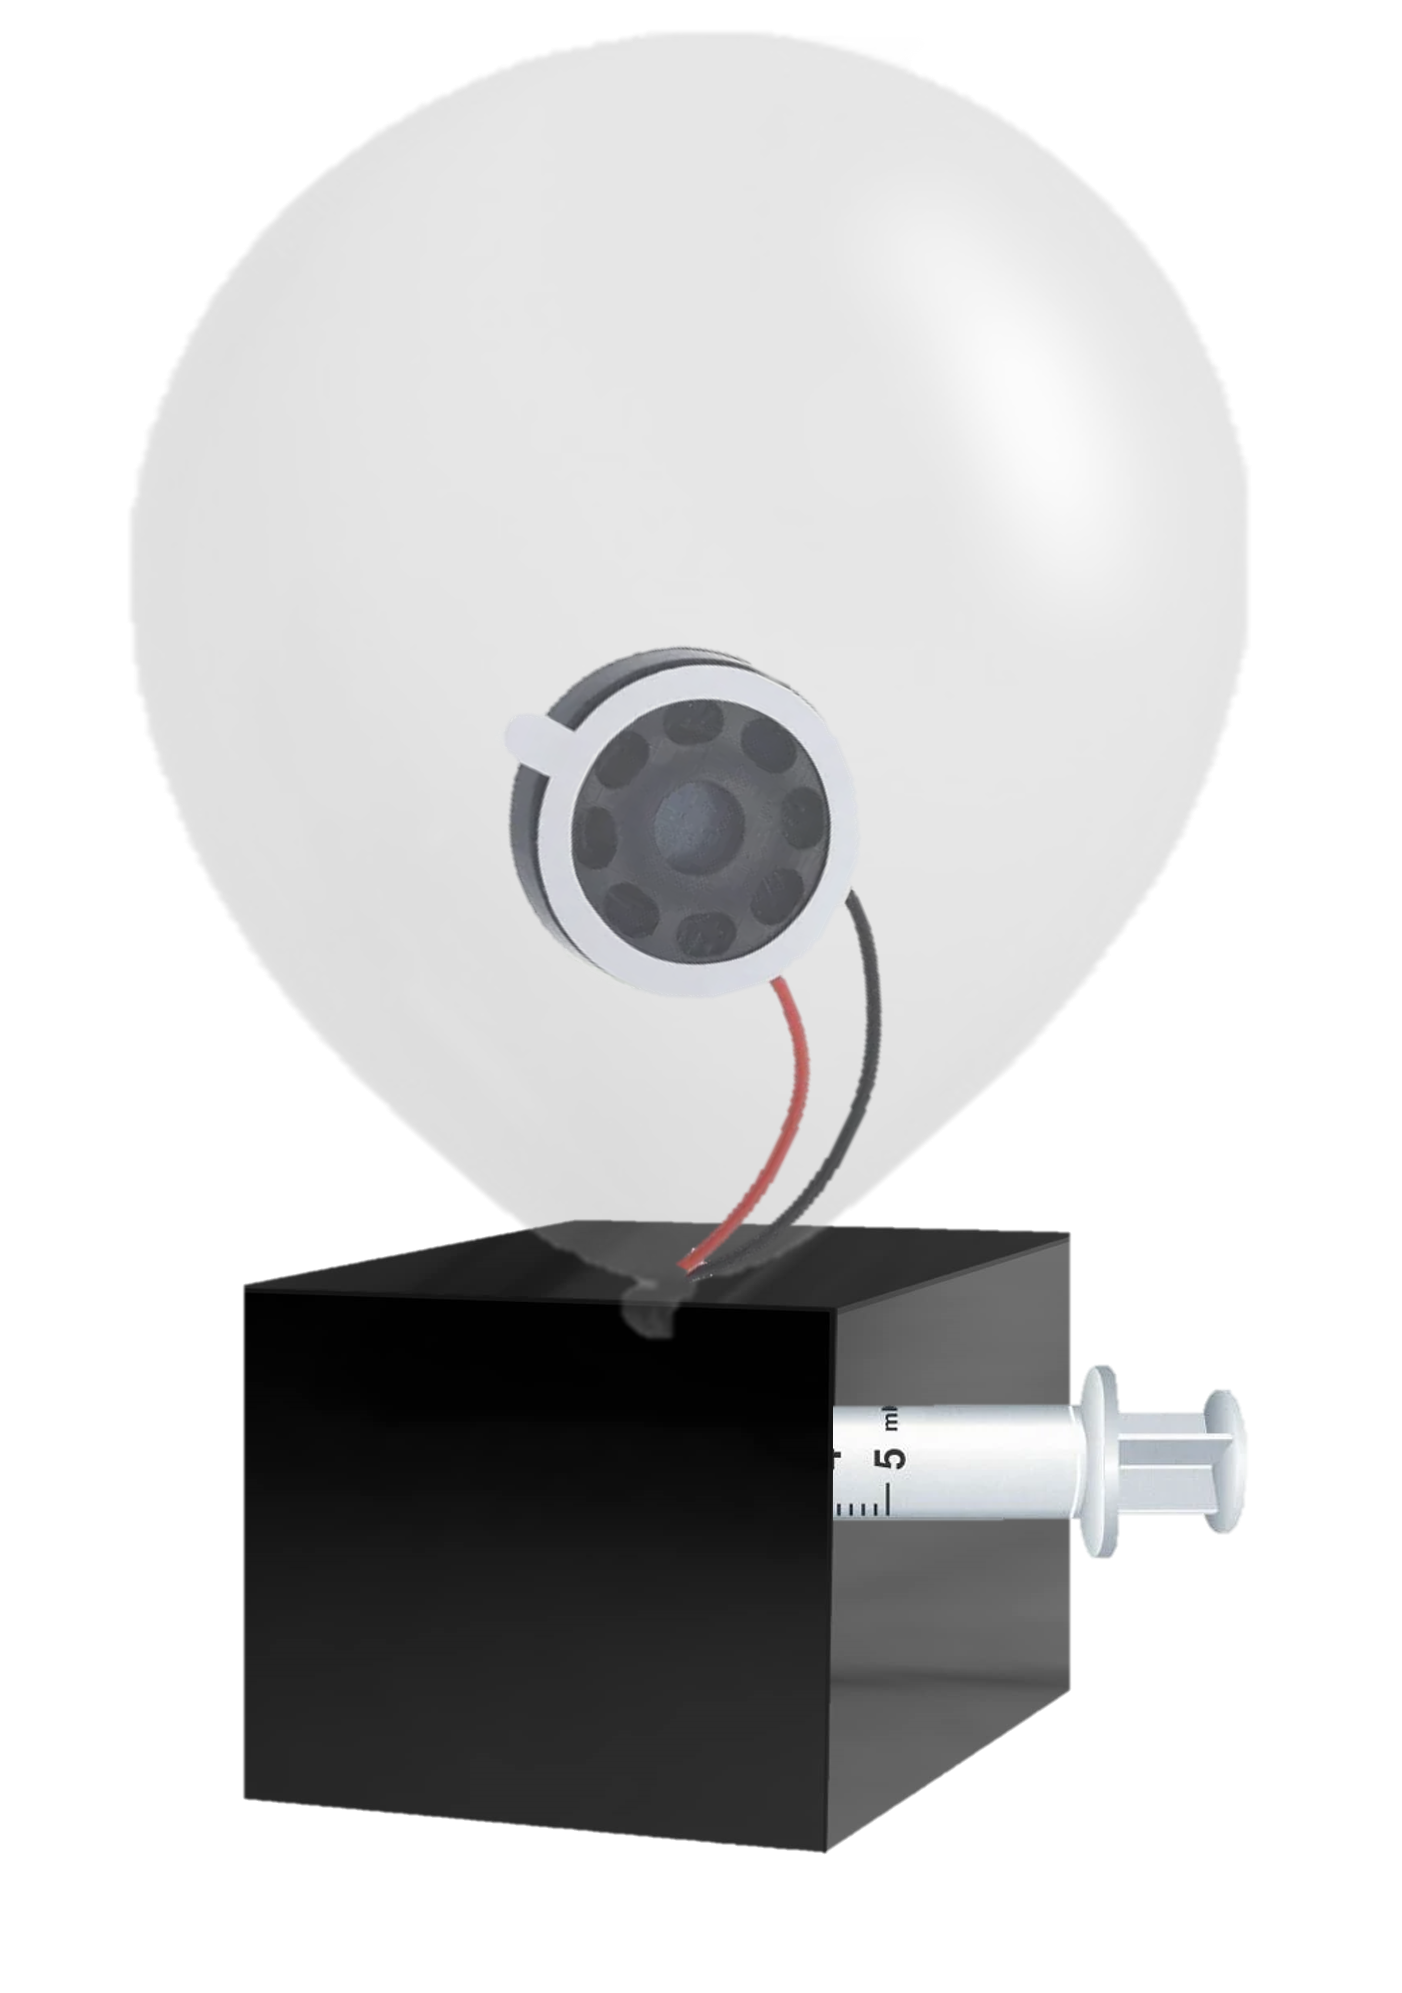
\includegraphics[scale=0.27]{figs/Phantom.png}
    \caption{Phantom to simulate heartbeat and breathing rates}
    \label{fig:phantom}
\end{figure}

For the development of a test object (Phantom), we are considering simulating the heartbeat using a speaker connected to recordings of heartbeats under normal and abnormal conditions, thus mimicking various heart-related conditions. This proposal is based on the displacement of the speaker's diaphragm according to the frequency of the audio being played. The speaker will be placed inside a latex balloon simulating a person's chest. To simulate movement, air will be introduced and withdrawn using a syringe directly connected to the balloon, allowing it to vary its volume at a specific and correlated frequency. This approach will enable us to represent various cardiac pathologies, such as Valsalva states or apnea.

\section{Detailed definition of the protocol followed to evaluate all the specifications}

\begin{enumerate}
    \item Frequency and Bandwidth antenna is according to resolution 115 of 23 March 2020  by Agencia Nacional del Espectro (ANE) \cite{ANERes105}. This specific that from 5725 to 5875 MHz  is part of ISM bands. In preliminary results will show the antenna design. 

    
    \item Measurement distance from the subject from 0 to 2 meters will be implemented with an appropriate power irradiation. 

    \item Real-time operation, heart rate, and respiration rate will be executed mostly by a USRP B200mini with the remaining system and computer. USRP B200mini programmed in Python allows signal processing to show in the frequency domain. Thus, the GUI computer is used to display graphic results.

    \item Presence or absence of a subject is done with radar running. That is if there are no signals of heart rate or respiration rate in the absence of a subject. In another case, between the two meters of range subject be present. 

    \item Error in heart rate and respiration rate is shown as the relative error where the actual value is the measurement with pulsometer, smartband, and simulated signals. 
     
    \item To achieve a false alarm rate for subject presence below 20 \%, the following measures are necessary: Use a transmission frequency that is significantly different from the respiratory rate and use a detection algorithm that takes into account the respiratory rate of the person. 

    \item Detection rate of subject presence 70 \%, this is achieved through several measurements, calibration, and integration in the algorithm.
    
\end{enumerate}


\section{Preliminary results}
\label{sec:prel_res}

Description of any design/simulation results obtained in the development of the project.

\subsection{Design specifications}

This is the first of several design tests to find an element with good resonance and penetration characteristics for the design of a penetration Doppler radar. For this first element, the required design specifications are the use of microstrip technology in a rectangular patch, reduced dimensions, shielding to improve isolation between the TX and RX antennas, powered by coaxial cable, 50 $\Omega$ input impedance, and cutoff frequency of 5.8 GHz.

\subsection{Technical specifications} 

Within the technical specifications, the antenna must have a resonance frequency of 5.8 GHz, the substrate must be made of FR4 material with a thickness (h) of 60 mil and have an input impedance of 50 $\Omega$, in addition to having a S11 greater than -10 dB, and shielding or shielding to help with the isolation between antennas.

Patch antenna is designed according to Figure \ref{fig:AntThe} and Equations \eqref{eq:des_w}, \eqref{eq:e_eff}, \eqref{eq:delta_L_h}, \eqref{eq:delta_L}, \eqref{eq:L_TM}, \eqref{eq:L_eff} y \eqref{eq:lambda_0}. Values given are:

\begin{itemize}
\item  $\epsilon_r=4.4$
\item $f_r=5.8 \; [GHz]$
\item $h=60 \; [mm]$

\end{itemize}

\begin{figure}[H]
\centering
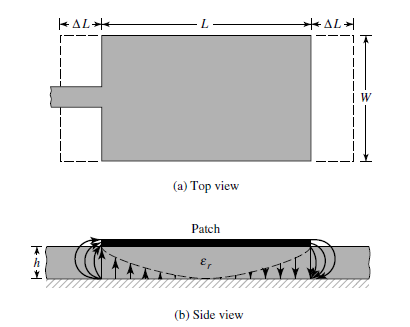
\includegraphics[width=0.7\linewidth]{figs/AntThe.png}
\caption{Patch antenna parameters. \cite{balanisAntennaTheoryAnalysis2005}}
\label{fig:AntThe}
\end{figure}

\begin{align}
\label{eq:des_w}
w =\frac{v_0}{2 f_r} \sqrt[2]{\frac{2}{\epsilon_r+1}}  =1.573 \; [cm]
\end{align}


\begin{align}
    \label{eq:e_eff}
    \epsilon_{reff} &= \frac{\epsilon_r+1}{2}+\frac{\epsilon_r-1}{2}\left[1+12\left(\frac{h}{w}\right)\right]^{-\frac{1}{2}} =3.856
\end{align}

\begin{align}
    \label{eq:delta_L_h}
    \frac{\Delta L}{h} &= 0.412 \left(\frac{\left(\epsilon_{reff}+0.3\right)\left(\frac{w}{h}+0.264\right)}{\left(\epsilon_{reff}-0.258\right)\left(\frac{w}{h}+0.8\right)} \right) 
\end{align}

\begin{align}
    \label{eq:delta_L}
    \Delta L = 0.06903 \; [cm]
\end{align}

\begin{align}
    \label{eq:L_TM}
    L_{TM010}=\frac{\lambda_d}{2}-2 \Delta L   =2.572 \; [cm]
\end{align}

\begin{align}
    \label{eq:L_eff}
    L_{eff}=L+2 \Delta L = 2.586+2\left(0.06903\right)=2.6\approx\frac{\lambda_d}{2}
\end{align}

\begin{align}
    \label{eq:lambda_0}
    \lambda_0=\frac{v_0}{f}=51.72 \; [mm]
\end{align}

\subsection{Design process} 
To carry out the design of the antenna, the Ansys Electronics Desktop Student software was used and the following stages were implemented for its design:

\begin{itemize}
\item Establish a previously calculated geometry.
\item Assign materials and radiation body.
\item Create an input port and specify a defined integration line for it.
\item Implement a solution with the required parameters.
\item Generate a parametric sweep and search for the closest solution.
\item Generate the results that are necessary for the analysis.
\end{itemize}

The design implemented in the antenna can be seen in Figure \ref{fig:Antenna}. In Figure \ref{fig:S11}, we can see the S11 parameter of the antenna designed in its version 1 for this proposal, which shows an attenuation of – 37 dB and a bandwidth of 140 MHz.In Figure \ref{fig:Parameter Z}, we can see the impedance parameter with Z=50.96-j0.50 $\Omega$.


\begin{figure}[H]
\centering
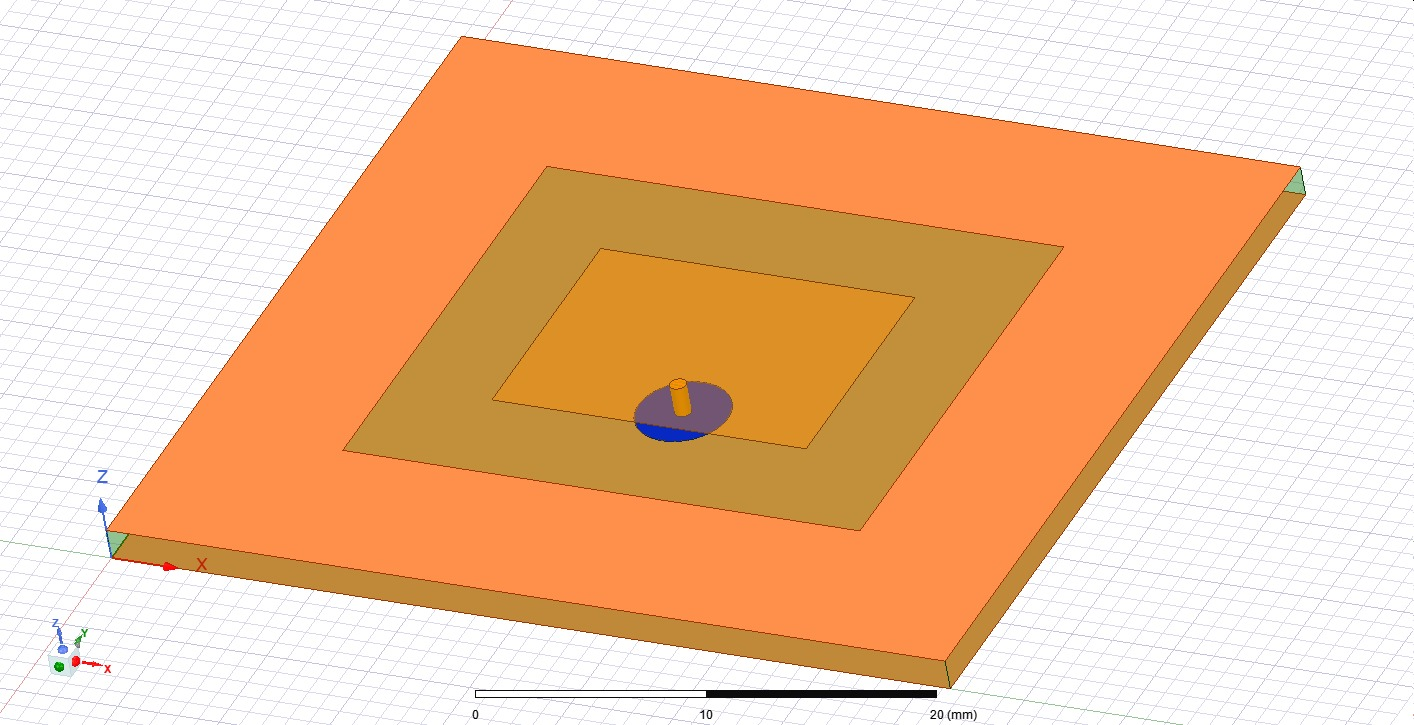
\includegraphics[width=0.5\linewidth]{figs/Antenna.jpeg}
\caption{3D antenna design.}
\label{fig:Antenna}
\end{figure}

\begin{figure}[H]
\centering
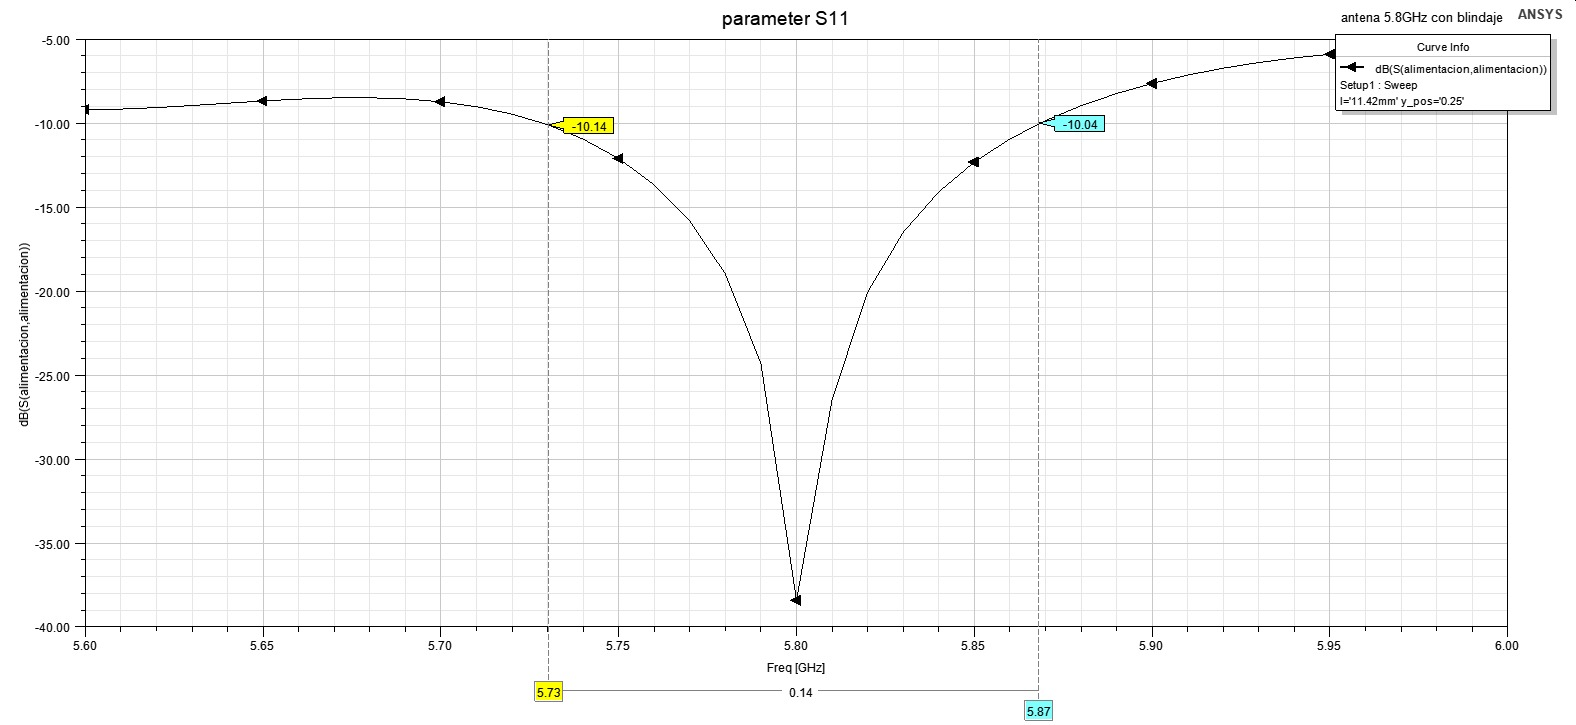
\includegraphics[width=0.7\linewidth]{figs/S11.jpeg}
\caption{Simulated S11 parameter.}
\label{fig:S11}
\end{figure}

\begin{figure}[H]
\centering
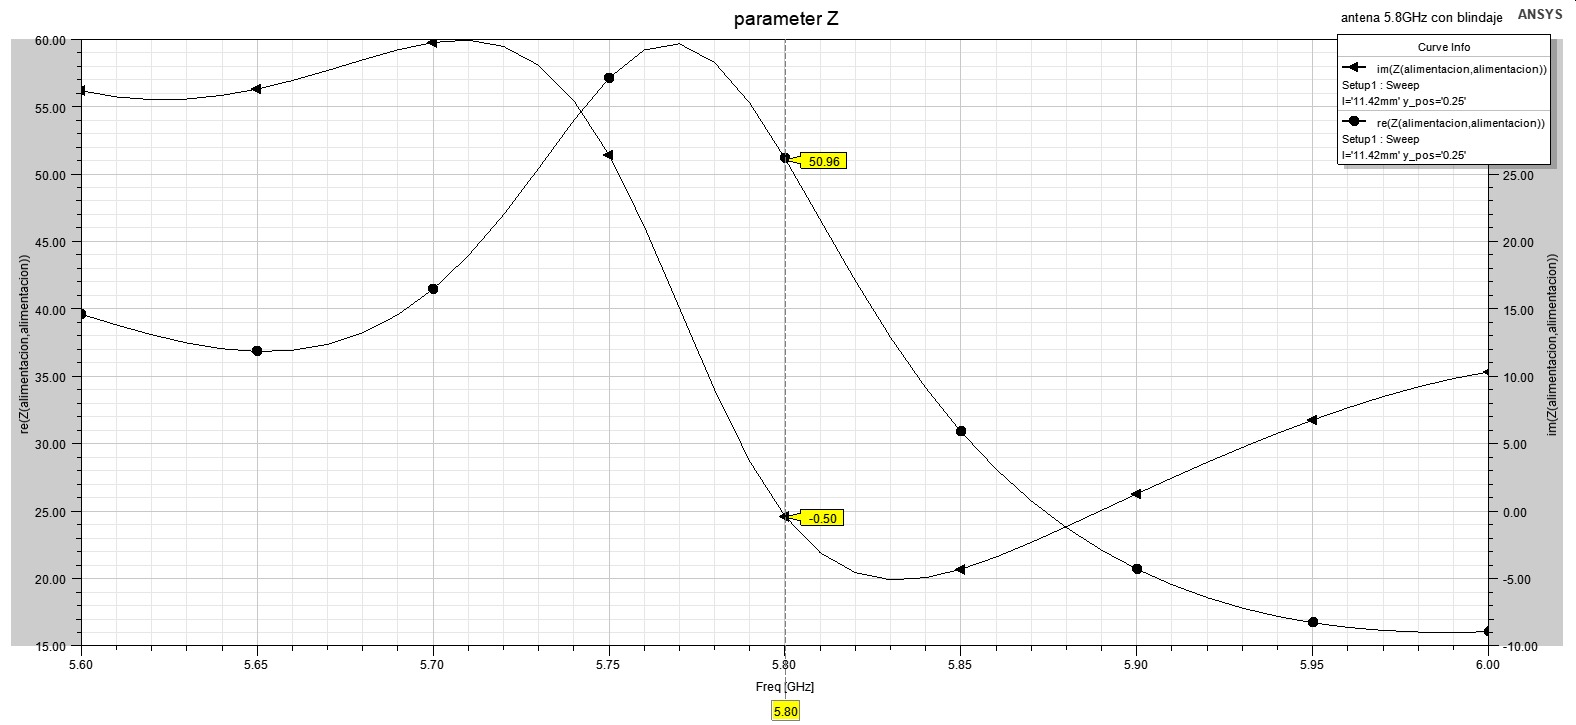
\includegraphics[width=0.7\linewidth]{figs/Parameter Z.jpeg}
\caption{Simulated Z parameter.}
\label{fig:Parameter Z}
\end{figure}



\section{Description of the challenges foreseen for the completion of the project and how these will be faced.}

One of the challenges we are considering is related to the reflective capacity of the speaker to simulate the heartbeat. While we can control the frequency at which radar data will be collected through this mechanism, the reflection capacity of the wave can be directly affected by two elements. The first of these is the membrane material, which is generally organic and its properties do not generate reflection in the incident radar wave and can even be transparent. In this regard, we are considering the possibility of coating the membrane with a material like thin aluminum, similar to paper, to make it more reflective. \\

Secondly, the output power of the speaker, although it should be low, presents challenges due to the mechanical and sensitivity conditions that can pose a problem if a minimum power is not considered to detect the movement of the speaker's membrane. This becomes even more critical when the membrane is possibly covered with an additional material for reflecting the electromagnetic wave that will impact it. To address this challenge, we will conduct characterization tests of the speaker, which will demonstrate the movement of the membrane according to input power, indicating a minimum at which the system will have the capacity to respond within the established design parameters.

\bibliographystyle{IEEEtran}
\bibliography{references}


% \begin{thebibliography}{1}
% \bibliographystyle{IEEEtran}

% \bibitem{kakouche}
% I. Kakouche, A. Maali, M. N. El Korso, A. Mesloub, M. S. Azzaz, "Fast and cost-effective method for non-contact respiration rate tracking using UWB impulse radar," Sensors and Actuators A: Physical, vol. 329, pp. 112814, 2021, \url{doi: 10.1016/j.sna.2021.112814.}

% \bibitem{ane_free_spectrum}
% Agencia Nacional del Espectro (2023, October 16). Gestión técnica. [Online]. Available: \url{https://www.ane.gov.co/SitePages/Gestión%20técnica/index.aspx?p=23}

% \bibitem{f.kraiemDopplerRadarArchitecture2019} 
% F. Kraiem, M. Dhieb, M. Ketata, H. Ghariani, y M. Lahiani, Doppler Radar Architecture for Vital Signal Detection, en 2019 IEEE International Conference on Design \& Test of Integrated Micro \& Nano-Systems (DTS), may 2019, pp. 1-5. doi: \url{10.1109/DTSS.2019.8915187.}

% \bibitem{ANERes105} Agencia Nacional del Espectro (ANE), Resolución No. 105 de 27 de marzo de 2020, ``Por medio de la cual se actualiza el Cuadro Nacional de Atribución de Bandas de Frecuencias''. República de Colombia, 2020.


% \bibitem{balanisAntennaTheoryAnalysis2005} C. A. Balanis, Antenna theory: analysis and design, 3rd ed. Hoboken, NJ: John Wiley, 2005.


% \end{thebibliography}



\end{document}

